\section{Code Runner}
\subsection{Overview}
\textbf{Code Runner} Component is a core component of Submission Worker Service, responsible for executing user-submitted programs against predefined test cases. It serves as a bridge between the user’s solution and the problem’s input–output data, ensuring fair and consistent evaluation. 
For each programming language supported by the platform (C++, Java, Python), a specific implementation of the \textbf{Code Runner} will be developed to handle language-specific compilation, execution, and output parsing. This ensures that user code is run correctly and consistently, regardless of the language chosen.
\subsection{Class Diagram}
\begin{figure}[h!]
    \centering
    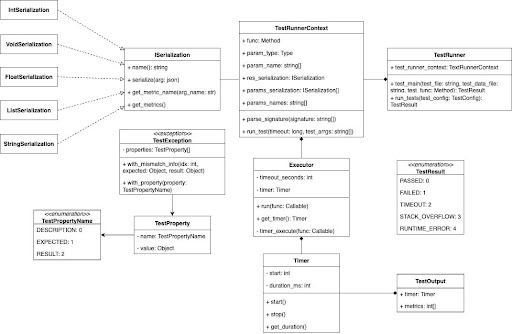
\includegraphics[width=1\textwidth]{Contents/Chapter 3/Code Runner/CodeRunner.jpg}
    \vspace{0.6cm}
    \caption{Class Diagram for Code Runner}
    \label{fig:leetcode-system}
\end{figure}

\begin{itemize}
    \item \textbf{ISerialization \& Implementations}: ISerialization defines a common interface for converting data between raw test inputs/outputs and program variables. Its implementations — IntSerialization, FloatSerialization, StringSerialization, ListSerialization, and VoidSerialization — handle serialization for different data types, ensuring test cases are interpreted correctly regardless of format.
    \item \textbf{TestRunnerContext}: TestRunnerContext stores the configuration and metadata needed to execute a user’s function, including parameter types, serializers, and the function reference itself. It prepares the environment for test execution and delegates the actual running to the Executor.
    \item \textbf{Executor}: Executor manages controlled execution of user-submitted functions. It enforces time limits, measures execution duration using Timer, and handles potential runtime issues like timeouts or errors during function calls.
    \item \textbf{Timer}: Timer measures how long each test case takes to execute. It provides simple start, stop, and duration tracking methods to record performance metrics for user solutions.
    \item \textbf{TestOutput}: TestOutput captures the results of a single test execution, storing both the runtime duration and any performance metrics. It is used to report how efficiently and accurately a user’s code performed.
    \item \textbf{TestException}: TestException represents errors or mismatches that occur during test execution. It stores details such as expected versus actual results and additional context through TestProperty objects.
    \item \textbf{TestProperty \& TestPropertyName}: TestProperty stores metadata about a test, such as a description or result comparison, identified by a TestPropertyName enum. These properties provide structured details for debugging failed test cases.
    \item \textbf{TestRunner}: TestRunner is the main controller responsible for running user code against predefined test cases. It coordinates between the TestRunnerContext, Executor, and ISerialization system to execute tests and produce final TestResult outcomes.
    \item \textbf{Solution}: Solution is the submission for the problem from the user.
\end{itemize}
\subsection{Testcase Format}
Each problem in the Online Judging System is accompanied by a test case file, named \textit{problem\_slug.csv}. This file defines a structured list of input–output test pairs used by the Test Runner of Worker Service to evaluate user submissions automatically.Moderators or superadmin upload this file when creating or updating a problem. The judging system parses the CSV, runs user code against each test case, and compares the output with the expected result.

To ensure accurate and consistent evaluation of user submissions, each input and output value in the \textit{problem\_slug.csv}file is associated with a data type. The type system defines how each field should be parsed, validated, and compared during the judging process.This mechanism helps the Test Framework interpret user program outputs correctly, whether they are numbers, strings, booleans, or lists. The following table describes the type.Here is the content for the "Problem Storages" section, including the table about type format:

\begin{table}[h!]
\centering
\renewcommand{\arraystretch}{1.3}
\begin{tabular}{|p{4cm}|p{10cm}|}
\hline
\textbf{Type Token} & \textbf{Description} \\ \hline

int & Integer numbers. \\ \hline

float & Floating-point numbers. \\ \hline

boolean & Boolean data. \\ \hline

string & Textual data. \\ \hline

void & Represents the absence of a value (e.g., for functions that return nothing). \\ \hline

list(type) & A collection of elements of a specified type (e.g., list(int)). \\ \hline

\end{tabular}
\caption{Data Types for Testcase Fields}
\end{table}
Each problem’s test case file will contain both type definitions for input, expected output and test data. The first line of the file specifies the data types for all inputs and outputs, helping the Test Runner correctly parse and validate values before running tests.

After executing all test cases for a user’s submission, the Test Runner generates a structured JSON result file summarizing the outcomes of each test. This file serves as the standardized output for the judging system and can be used by other services (such as the Result Service or API Gateway) to record, display, or analyze user performance. The JSON format ensures that results are machine-readable, language-independent, and easy to integrate into the overall online judging pipeline. The exported JSON file contains both metadata (e.g., problem name, language, execution status) and detailed per-test results (e.g., input, output, expected result, duration, and status).
